\chapter{Cart Pole}
\label{chap:cartpole}
In questo capitolo cerchiamo di risolvere l’ambiente Cart Pole, introdotto nella Sezione \ref{sec:cartpole}.

Per verificare il raggiungimento dell’obiettivo, abbiamo considerato un ritorno medio per episodio di almeno 475 punti. Il comportamento dell’agente viene osservato tramite un grafico che mostra la somma delle ricompense per epoca; a causa del forte rumore, il grafico è stato rappresentato utilizzando una media mobile esponenziale (Time Weighted EMA) con fattore 0{,}95. Questa scelta consente di generalizzare anche ad altri ambienti, come vedremo nel prossimo capitolo.

%%%%%%%%%%%%%%%%%%%%%%%%%%%%%%%%%%%%%%%%%%%%%%%%
\section{Baseline}
In questa sezione analizziamo diverse strategie di baseline. Siamo partiti da un’implementazione di REINFORCE senza baseline, proseguendo con una standardizzazione dei returns e infine con una stima della funzione di valore dello stato.

%%%%%%%%%%%%%%%%%%%%%
\subsection{Nessuna baseline}
I primi esperimenti sono stati condotti senza alcuna baseline.

\myskip

Come si osserva nella Figura \ref{fig:returnsno}, senza baseline l’apprendimento risulta molto irregolare e, anche dopo 3000 episodi, l’ambiente non viene risolto in modo stabile; solo il primo esperimento si avvicina a una possibile soluzione. Le tre iterazioni mostrano risultati piuttosto differenti.

\begin{figure}[htbp]
\centering
\begin{subfigure}{0.45\textwidth}
\centering
\includegraphics[width=\textwidth]{immages/3-cart pole/returns.pdf}
\caption{Somma delle ricompense}
\label{fig:returnsno}
\end{subfigure}
\hfill
\begin{subfigure}{0.45\textwidth}
\centering
\includegraphics[width=\textwidth]{immages/3-cart pole/loss.pdf}
\caption{Loss}
\label{fig:lossno}
\end{subfigure}
\caption{Esperimenti senza baseline.}
\end{figure}

\myskip

Un’osservazione interessante riguarda la loss: come mostrato in Figura \ref{fig:lossno}, questa è altamente irregolare e non mostra un andamento decrescente tipico dell’apprendimento supervisionato. Ciò deriva dalla natura stocastica dell’algoritmo: i returns variano a ogni episodio e influenzano direttamente la loss, che è anch’essa funzione della policy, aggiornata a ogni episodio.

%%%%%%%%%%%%%%%%%%%%%
\subsection{Standardizzazione}
Per migliorare la stabilità dell’apprendimento, abbiamo standardizzato i returns all’interno di ogni episodio.

\myskip

Come mostrato in Figura \ref{fig:returnsstd}, questa tecnica produce un apprendimento più regolare. L’ambiente viene risolto intorno ai 1500 episodi, con somme delle ricompense costantemente superiori a 475.

\begin{figure}[htbp]
\centering
\begin{subfigure}{0.45\textwidth}
\centering
\includegraphics[width=\textwidth]{immages/3-cart pole/returns_std.pdf}
\caption{Ricompense standardizzate}
\label{fig:returnsstd}
\end{subfigure}
\hfill
\begin{subfigure}{0.45\textwidth}
\centering
\includegraphics[width=\textwidth]{immages/3-cart pole/loss_std.pdf}
\caption{Loss}
\label{fig:lossstd}
\end{subfigure}
\caption{Esperimenti con standardizzazione.}
\end{figure}

\myskip

Osservando la loss in Figura \ref{fig:lossstd}, notiamo che i suoi valori sono contenuti in un intervallo ristretto attorno a $\pm1$, effetto diretto della standardizzazione dei returns.

%%%%%%%%%%%%%%%%%%%%%
\subsection{Baseline con funzione di valore}
In questo caso, la baseline è rappresentata dalla funzione di valore dello stato, approssimata da una rete neurale con la stessa architettura di quella della policy.

\myskip

Questa tecnica rende gli esperimenti più prevedibili, con risultati meno variabili tra le esecuzioni, come mostrato in Figura \ref{fig:returnsstate}.

\begin{figure}[htbp]
\centering
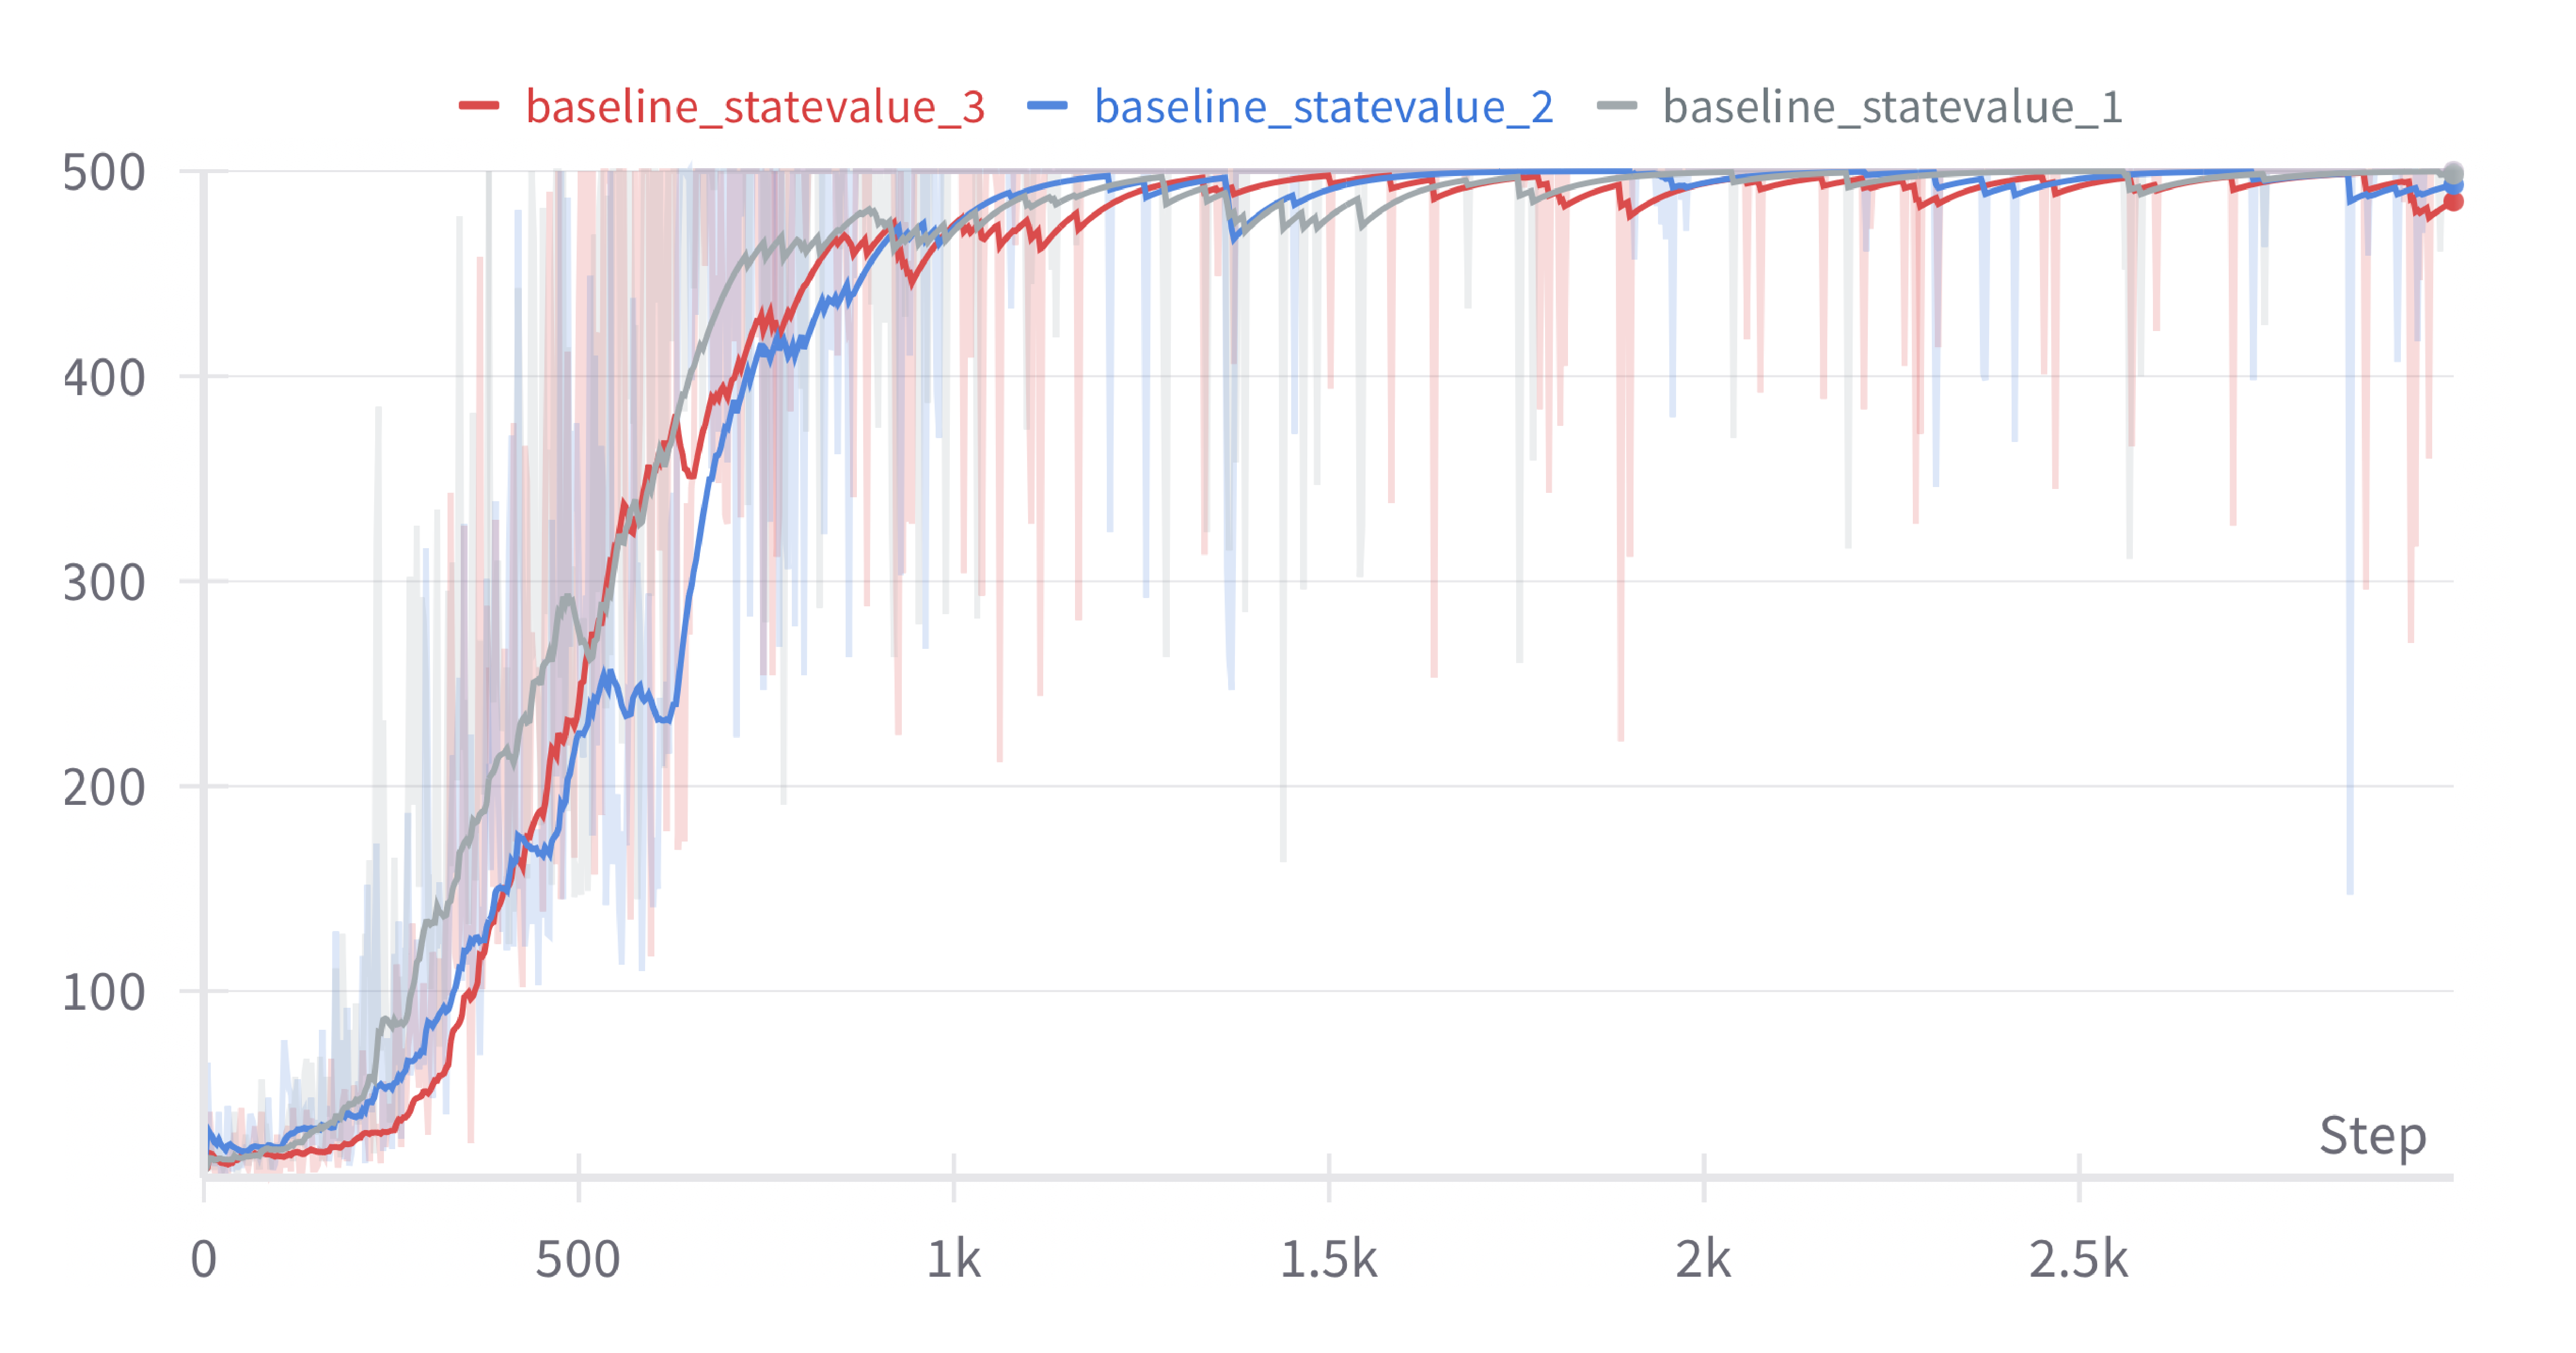
\includegraphics[width=.9\textwidth]{immages/3-cart pole/returns_state.pdf}
\caption{Ricompense con baseline state-value function.}
\label{fig:returnsstate}
\end{figure}

\myskip

Il confronto con la standardizzazione (Figura \ref{fig:confronto}) mostra che questa tecnica offre maggiore stabilità e una migliore velocità di convergenza.

Dal punto di vista computazionale (Figura \ref{fig:time}), l’implementazione senza baseline è la più veloce, mentre l’approssimazione della funzione di valore è la più lenta.

\begin{figure}[htbp]
\centering
\begin{subfigure}{0.45\textwidth}
\centering
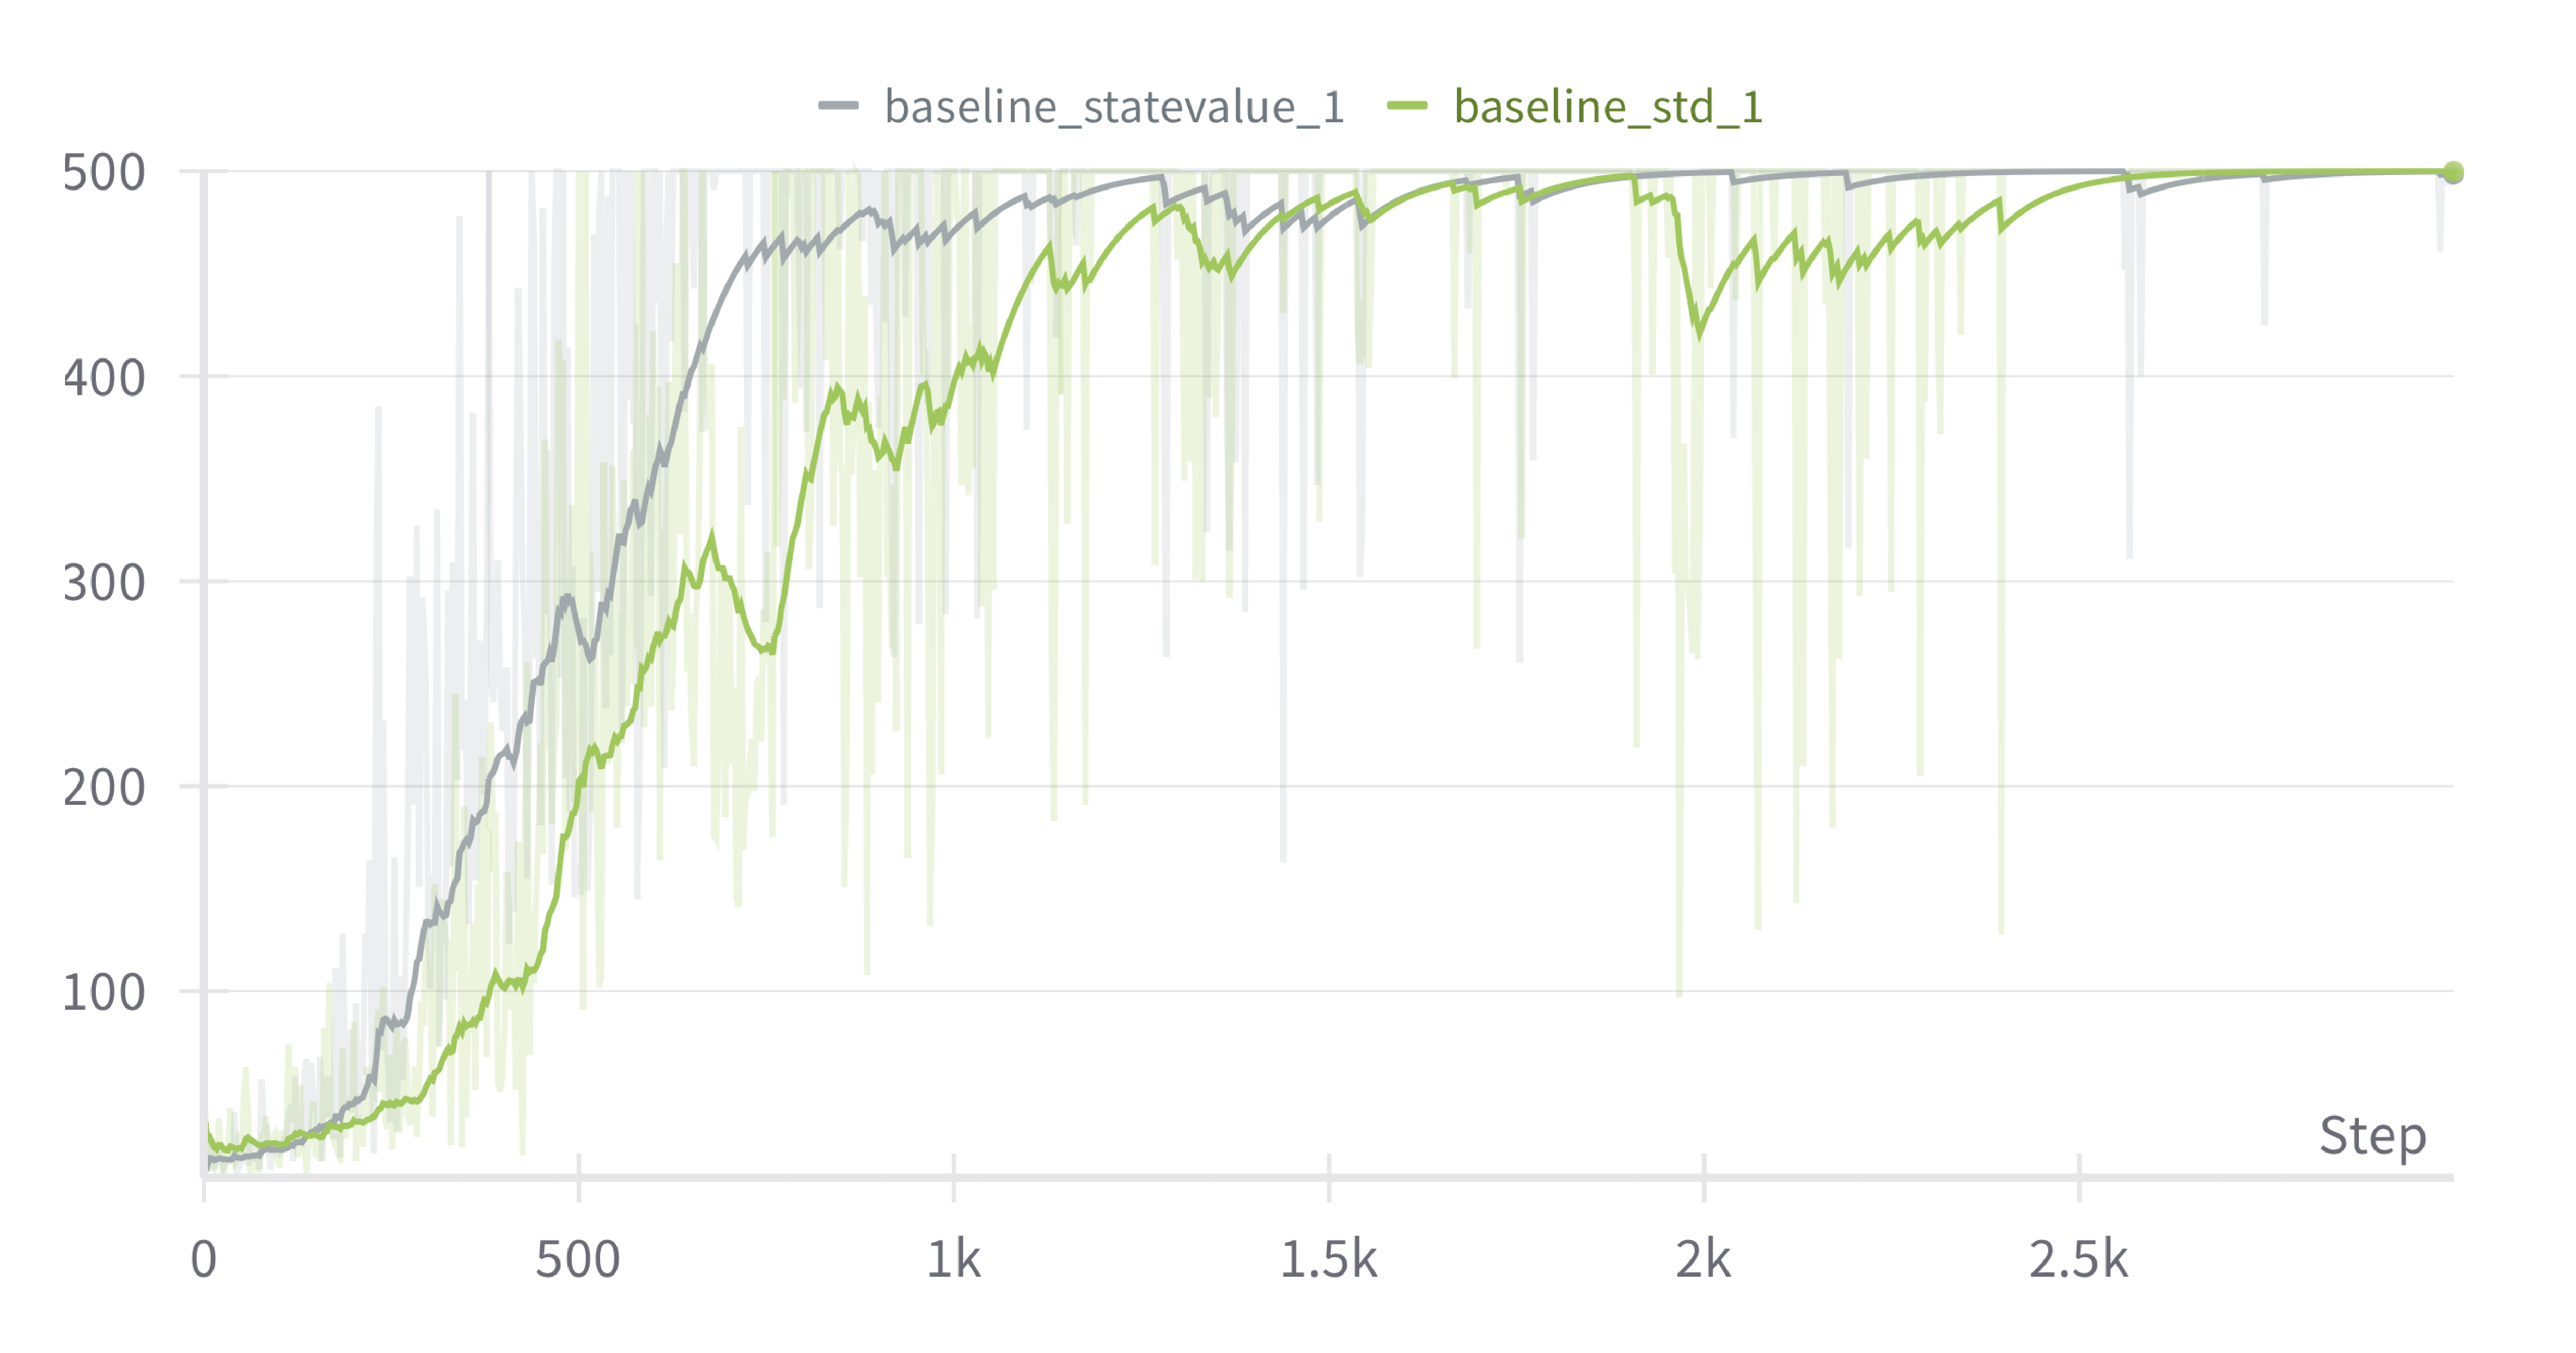
\includegraphics[width=.9\textwidth]{immages/3-cart pole/confronto_returns.pdf}
\caption{Confronto ricompense}
\label{fig:confronto}
\end{subfigure}
\hfill
\begin{subfigure}{0.45\textwidth}
\centering
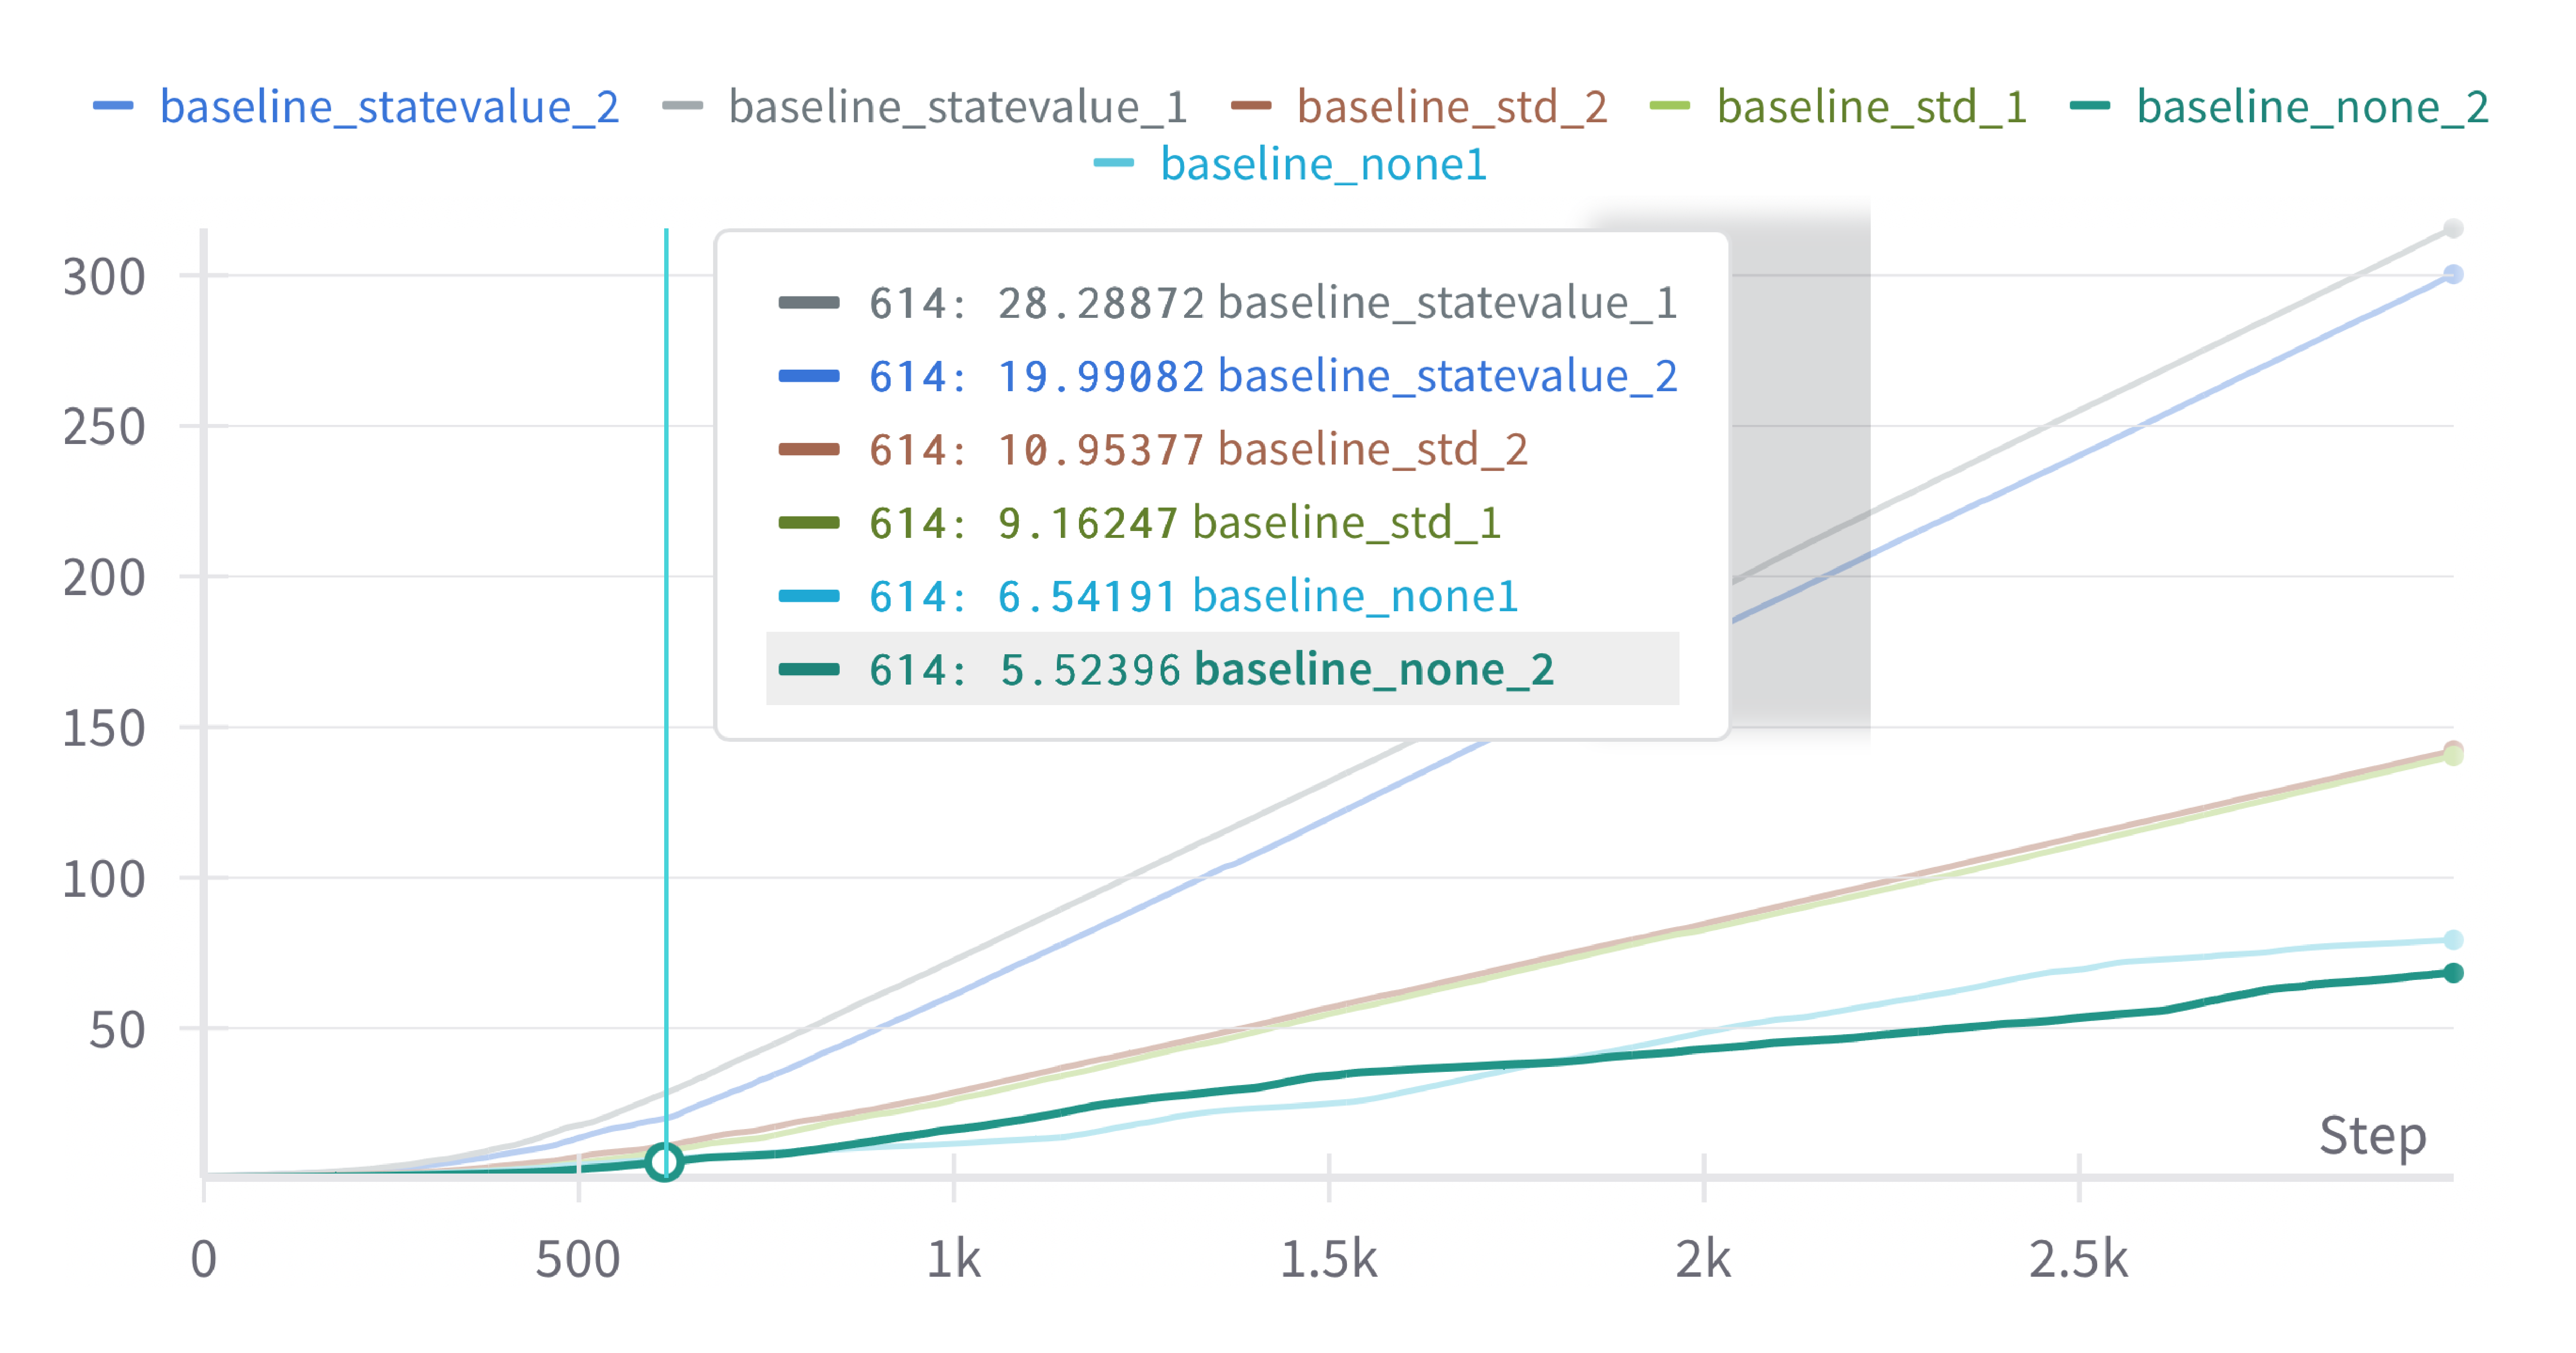
\includegraphics[width=\textwidth]{immages/3-cart pole/time.pdf}
\caption{Tempi di esecuzione}
\label{fig:time}
\end{subfigure}
\caption{Confronto tra le tecniche.}
\end{figure}

\myskip

Analizzando la loss della policy (Figura \ref{fig:lossstate}), si nota un andamento inizialmente simile al caso senza baseline, ma che con il progredire degli episodi tende a convergere.

\begin{figure}[htbp]
\centering
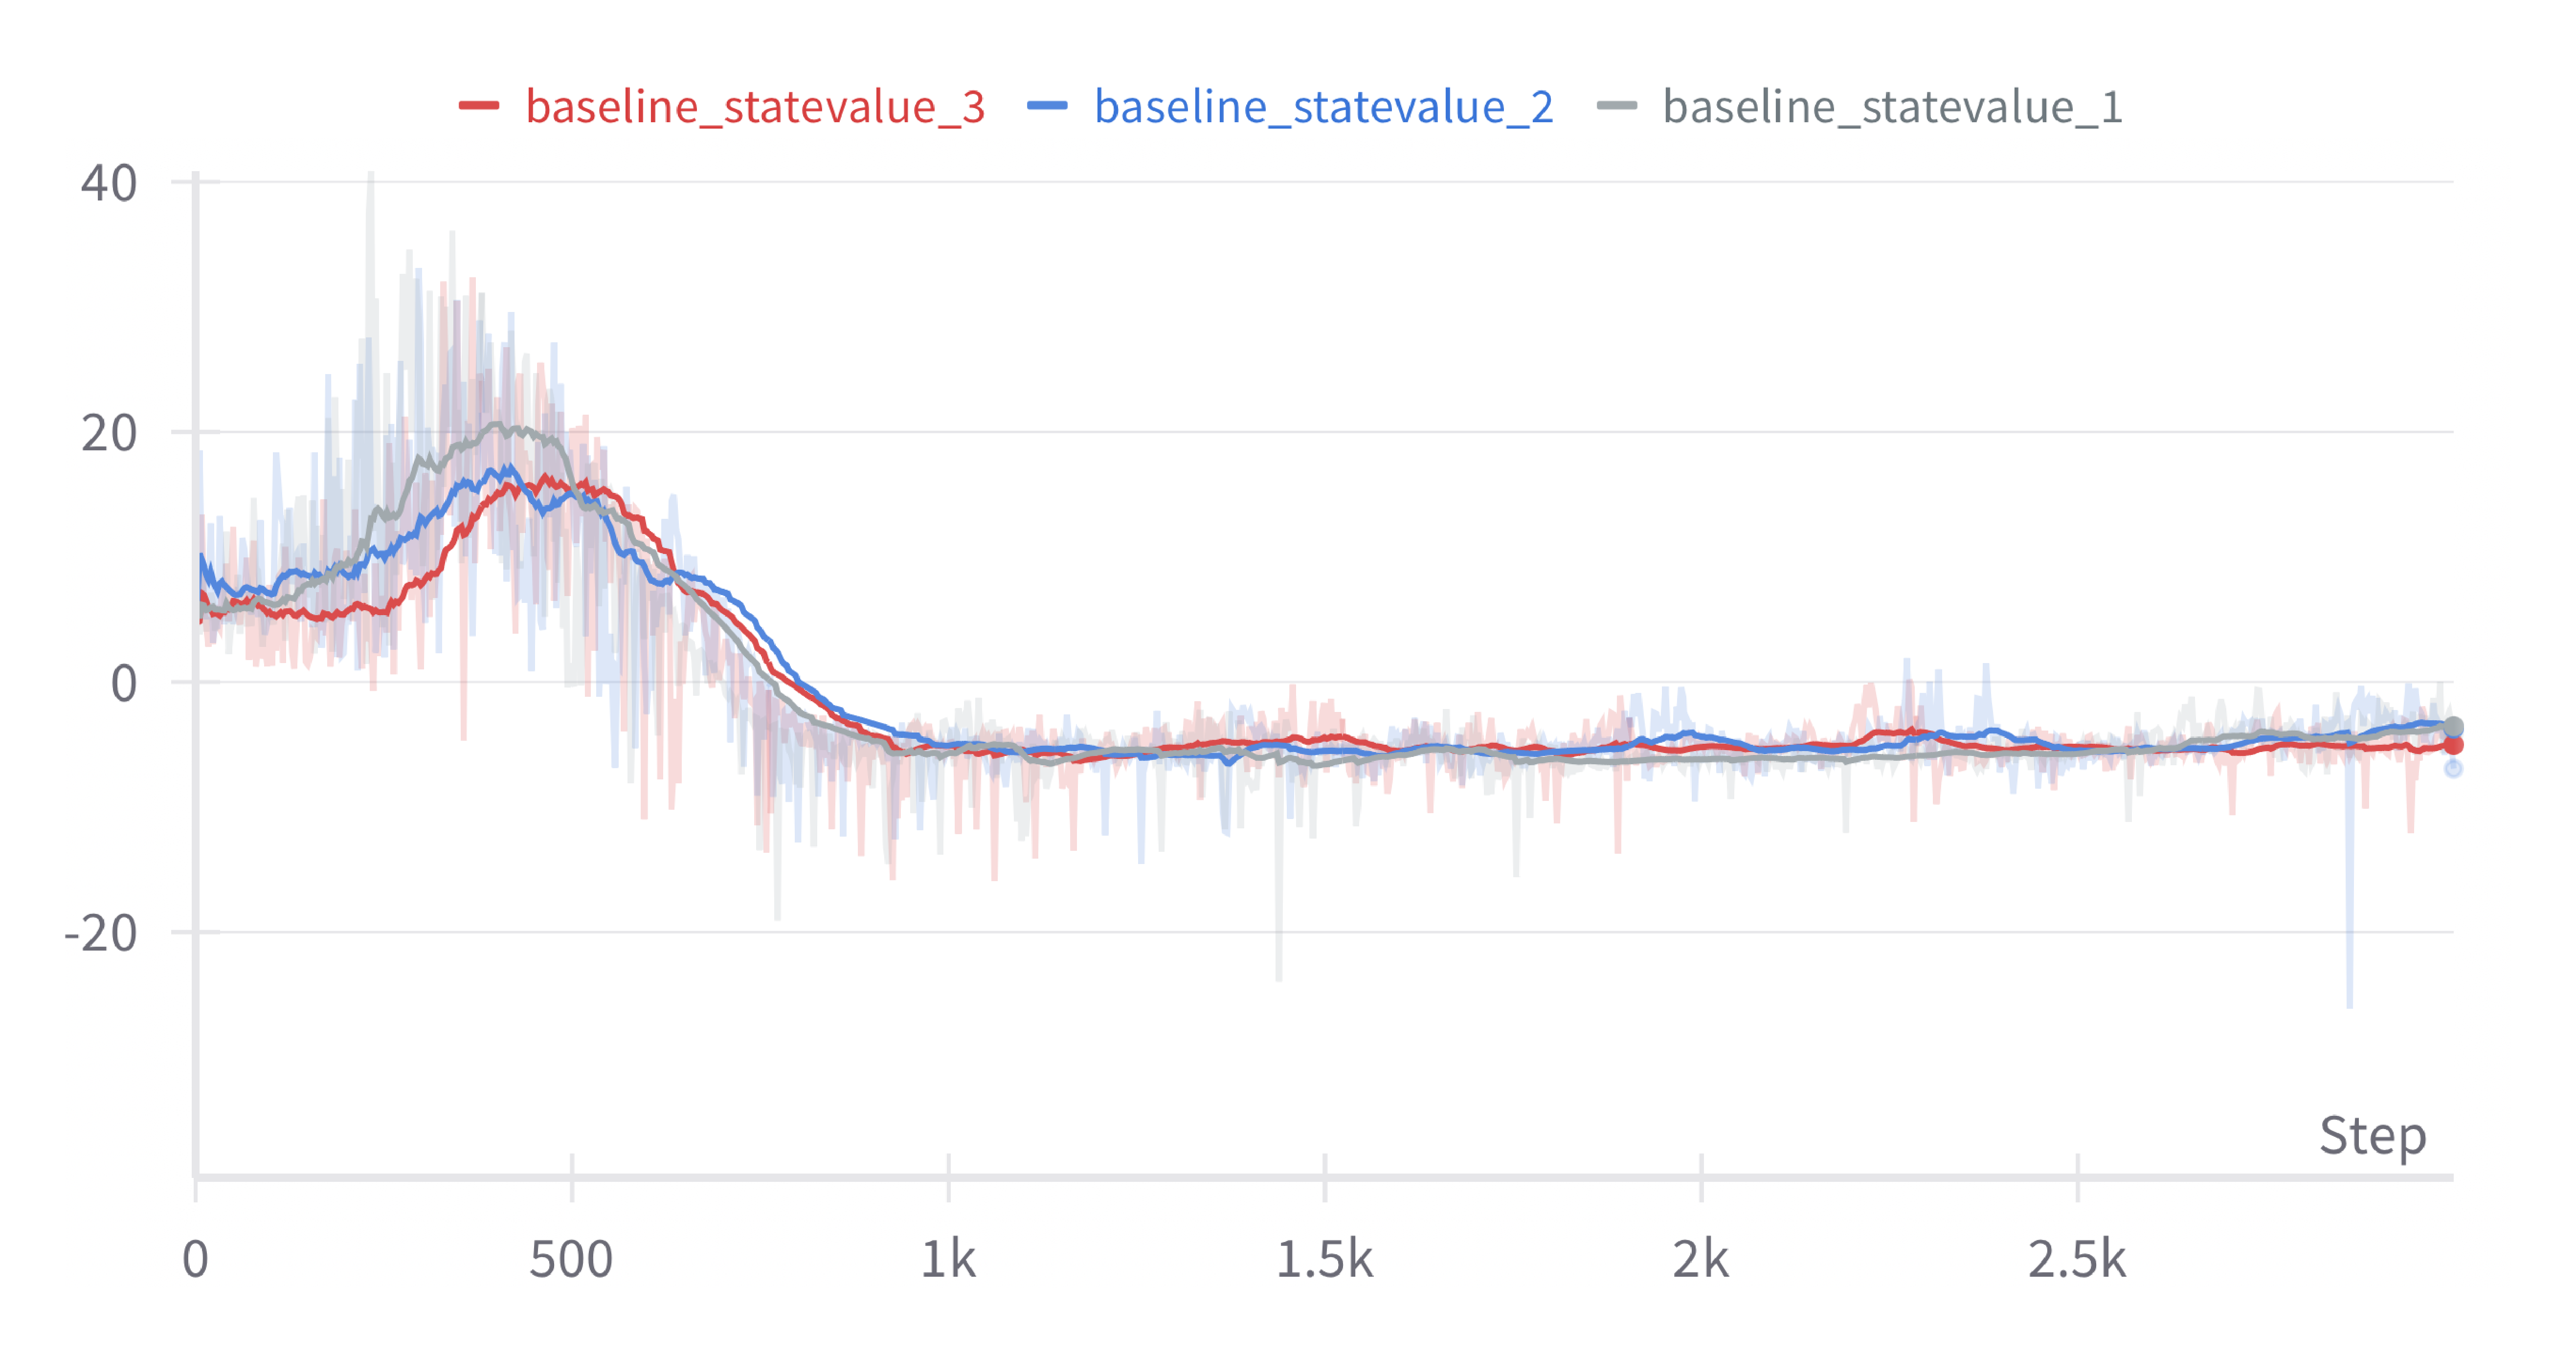
\includegraphics[width=.9\textwidth]{immages/3-cart pole/loss_state.pdf}
\caption{Loss della policy con baseline state-value function.}
\label{fig:lossstate}
\end{figure}

%%%%%%%%%%%%%%%%%%%%%%%%%%%%%%%%%%%%%%%%%%%%%%%%
\section{Iperparametri}
Finora, il fattore di sconto $\gamma$ e il learning rate sono stati impostati rispettivamente a 0{,}99 e 1e-3. In questa sezione analizziamo l’effetto della loro variazione. I valori esplorati sono: $\gamma$ tra 0{,}9 e 0{,}999 e learning rate tra 1e-5 e 1e-2. La baseline utilizzata è l’approssimazione della funzione di valore.

\myskip

Il grafico principale di riferimento resta quello della somma dei returns per epoca, filtrato con una Time Weighted EMA con fattore 0{,}99.

\myskip

La Figura \ref{fig:gammabasso} mostra tre esperimenti con learning rate molto basso (circa 1e-5) e $\gamma$ tra 0{,}93 e 0{,}97. L’agente non riesce ad apprendere.

\begin{figure}[htbp]
\centering
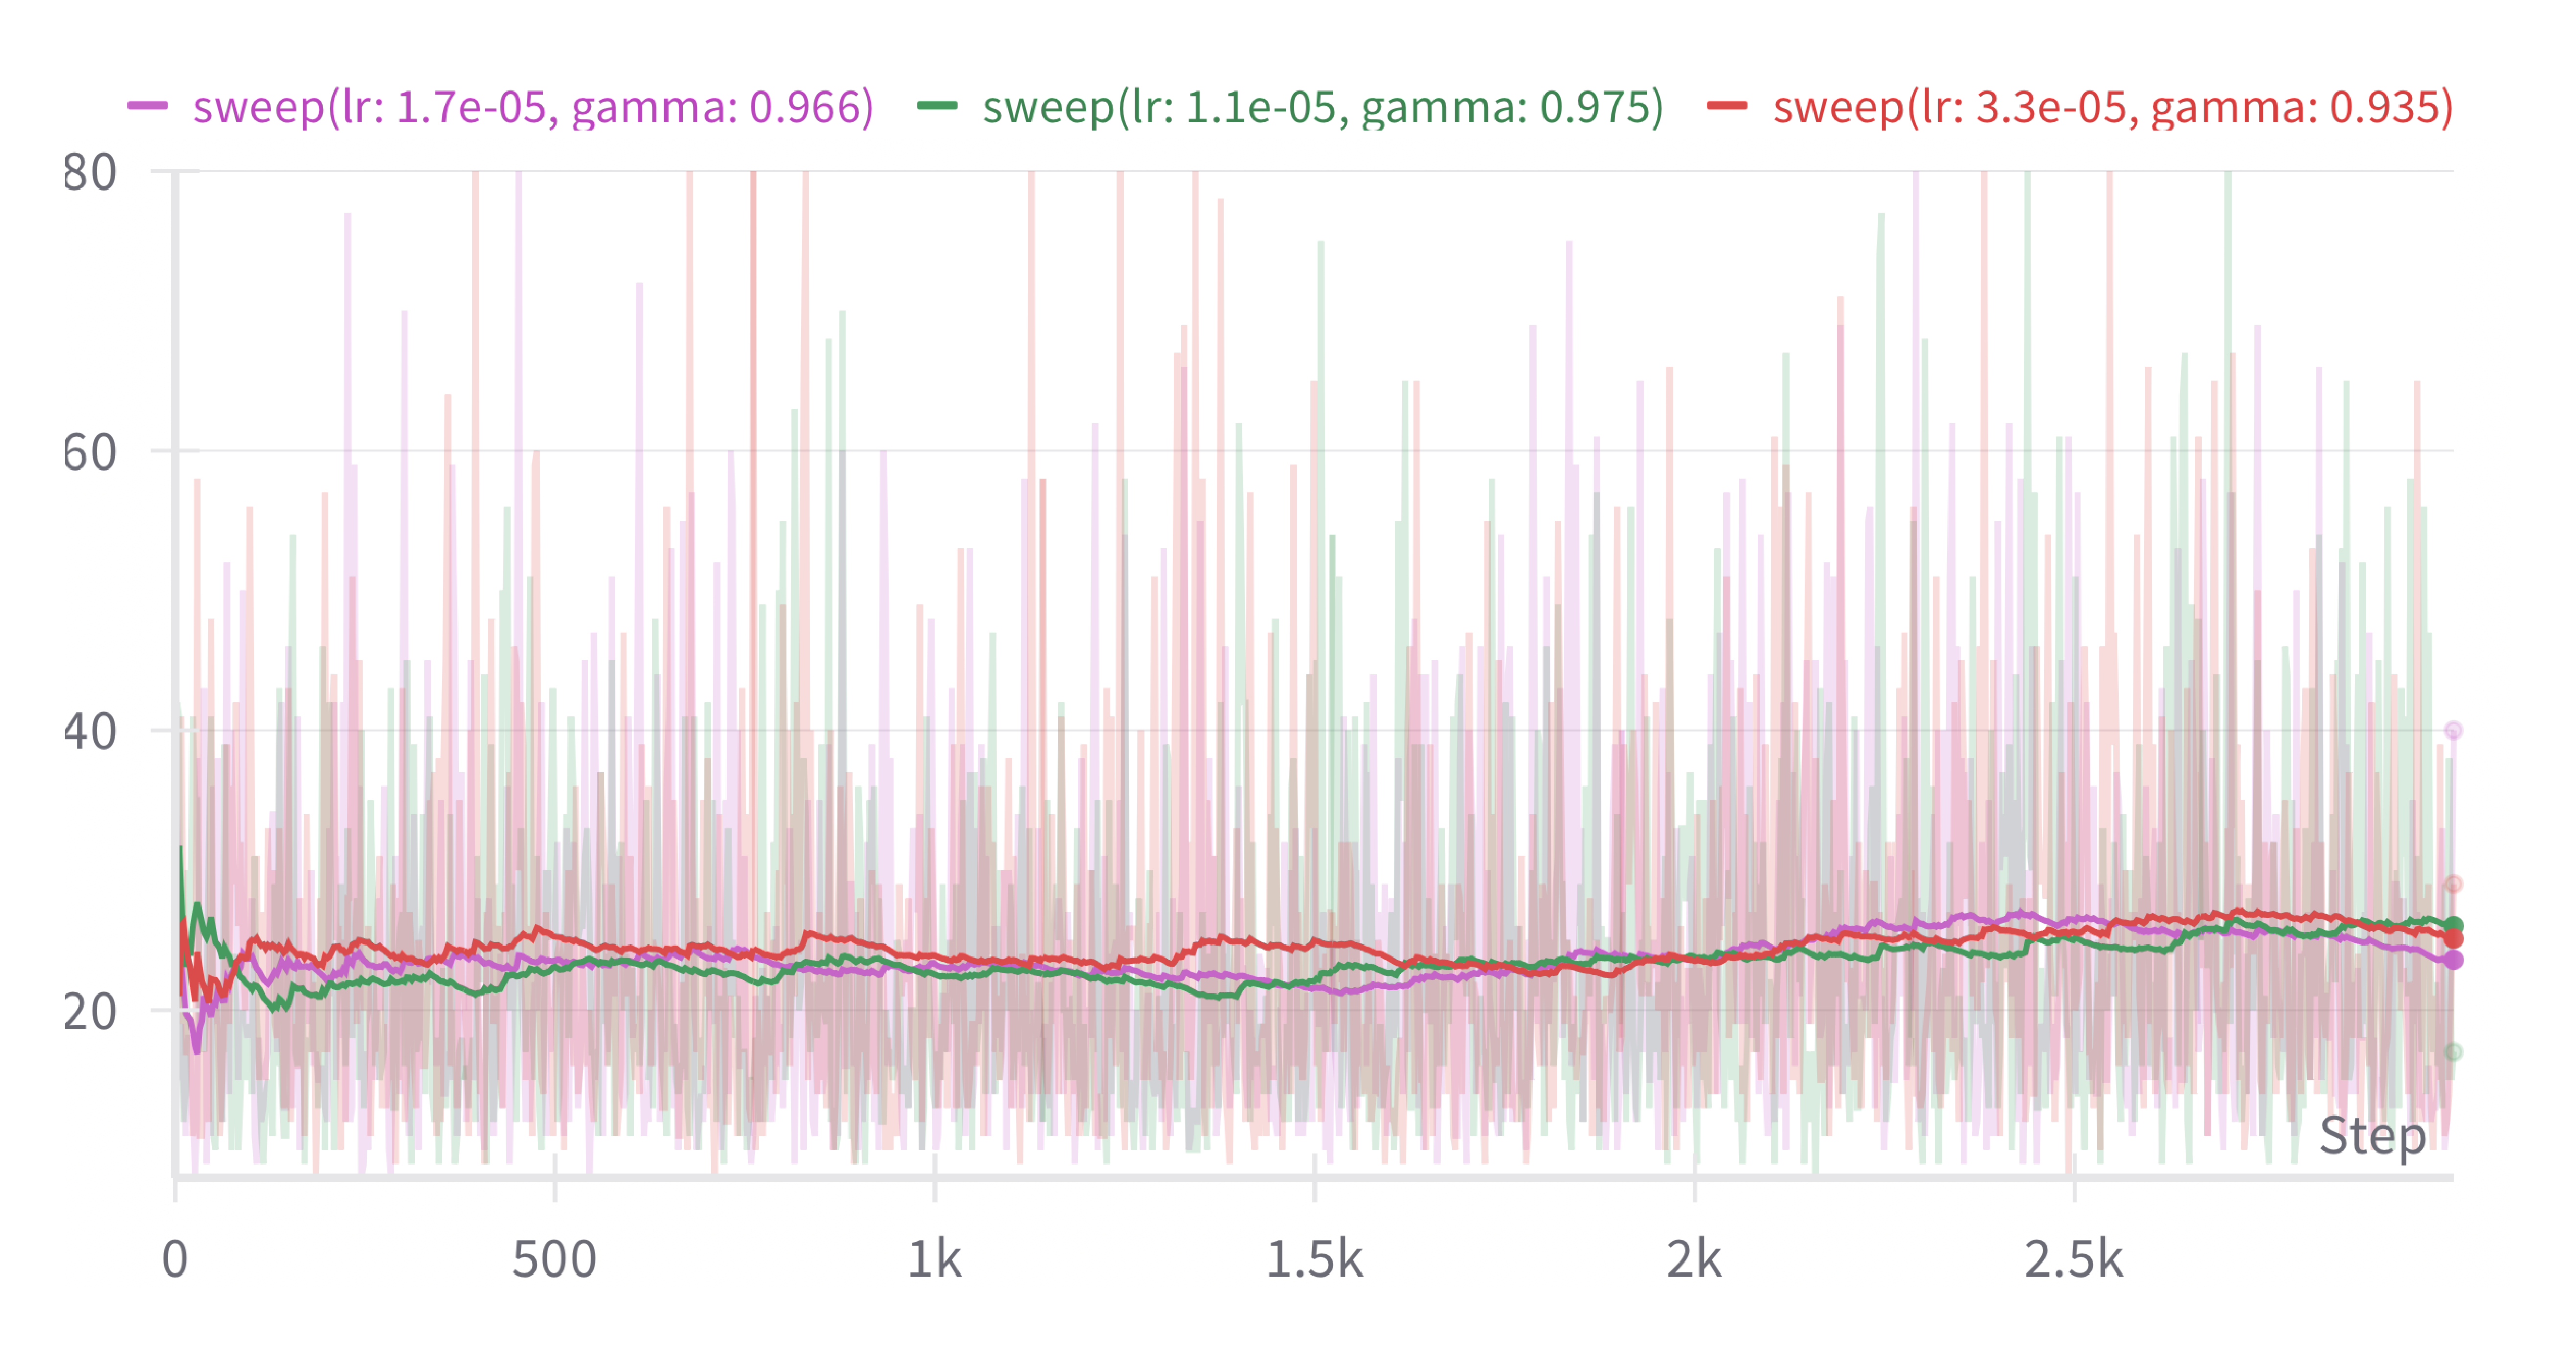
\includegraphics[width=.9\textwidth]{immages/3-cart pole/lr_basso.pdf}
\caption{Learning rate circa 1e-5.}
\label{fig:gammabasso}
\end{figure}

\myskip

La Figura \ref{fig:ampiorange} raccoglie altri esperimenti con combinazioni diverse. I migliori risultati si ottengono con $\gamma$ elevati, confermando la sensibilità dell’algoritmo REINFORCE a questi iperparametri.

\begin{figure}[htbp]
\centering
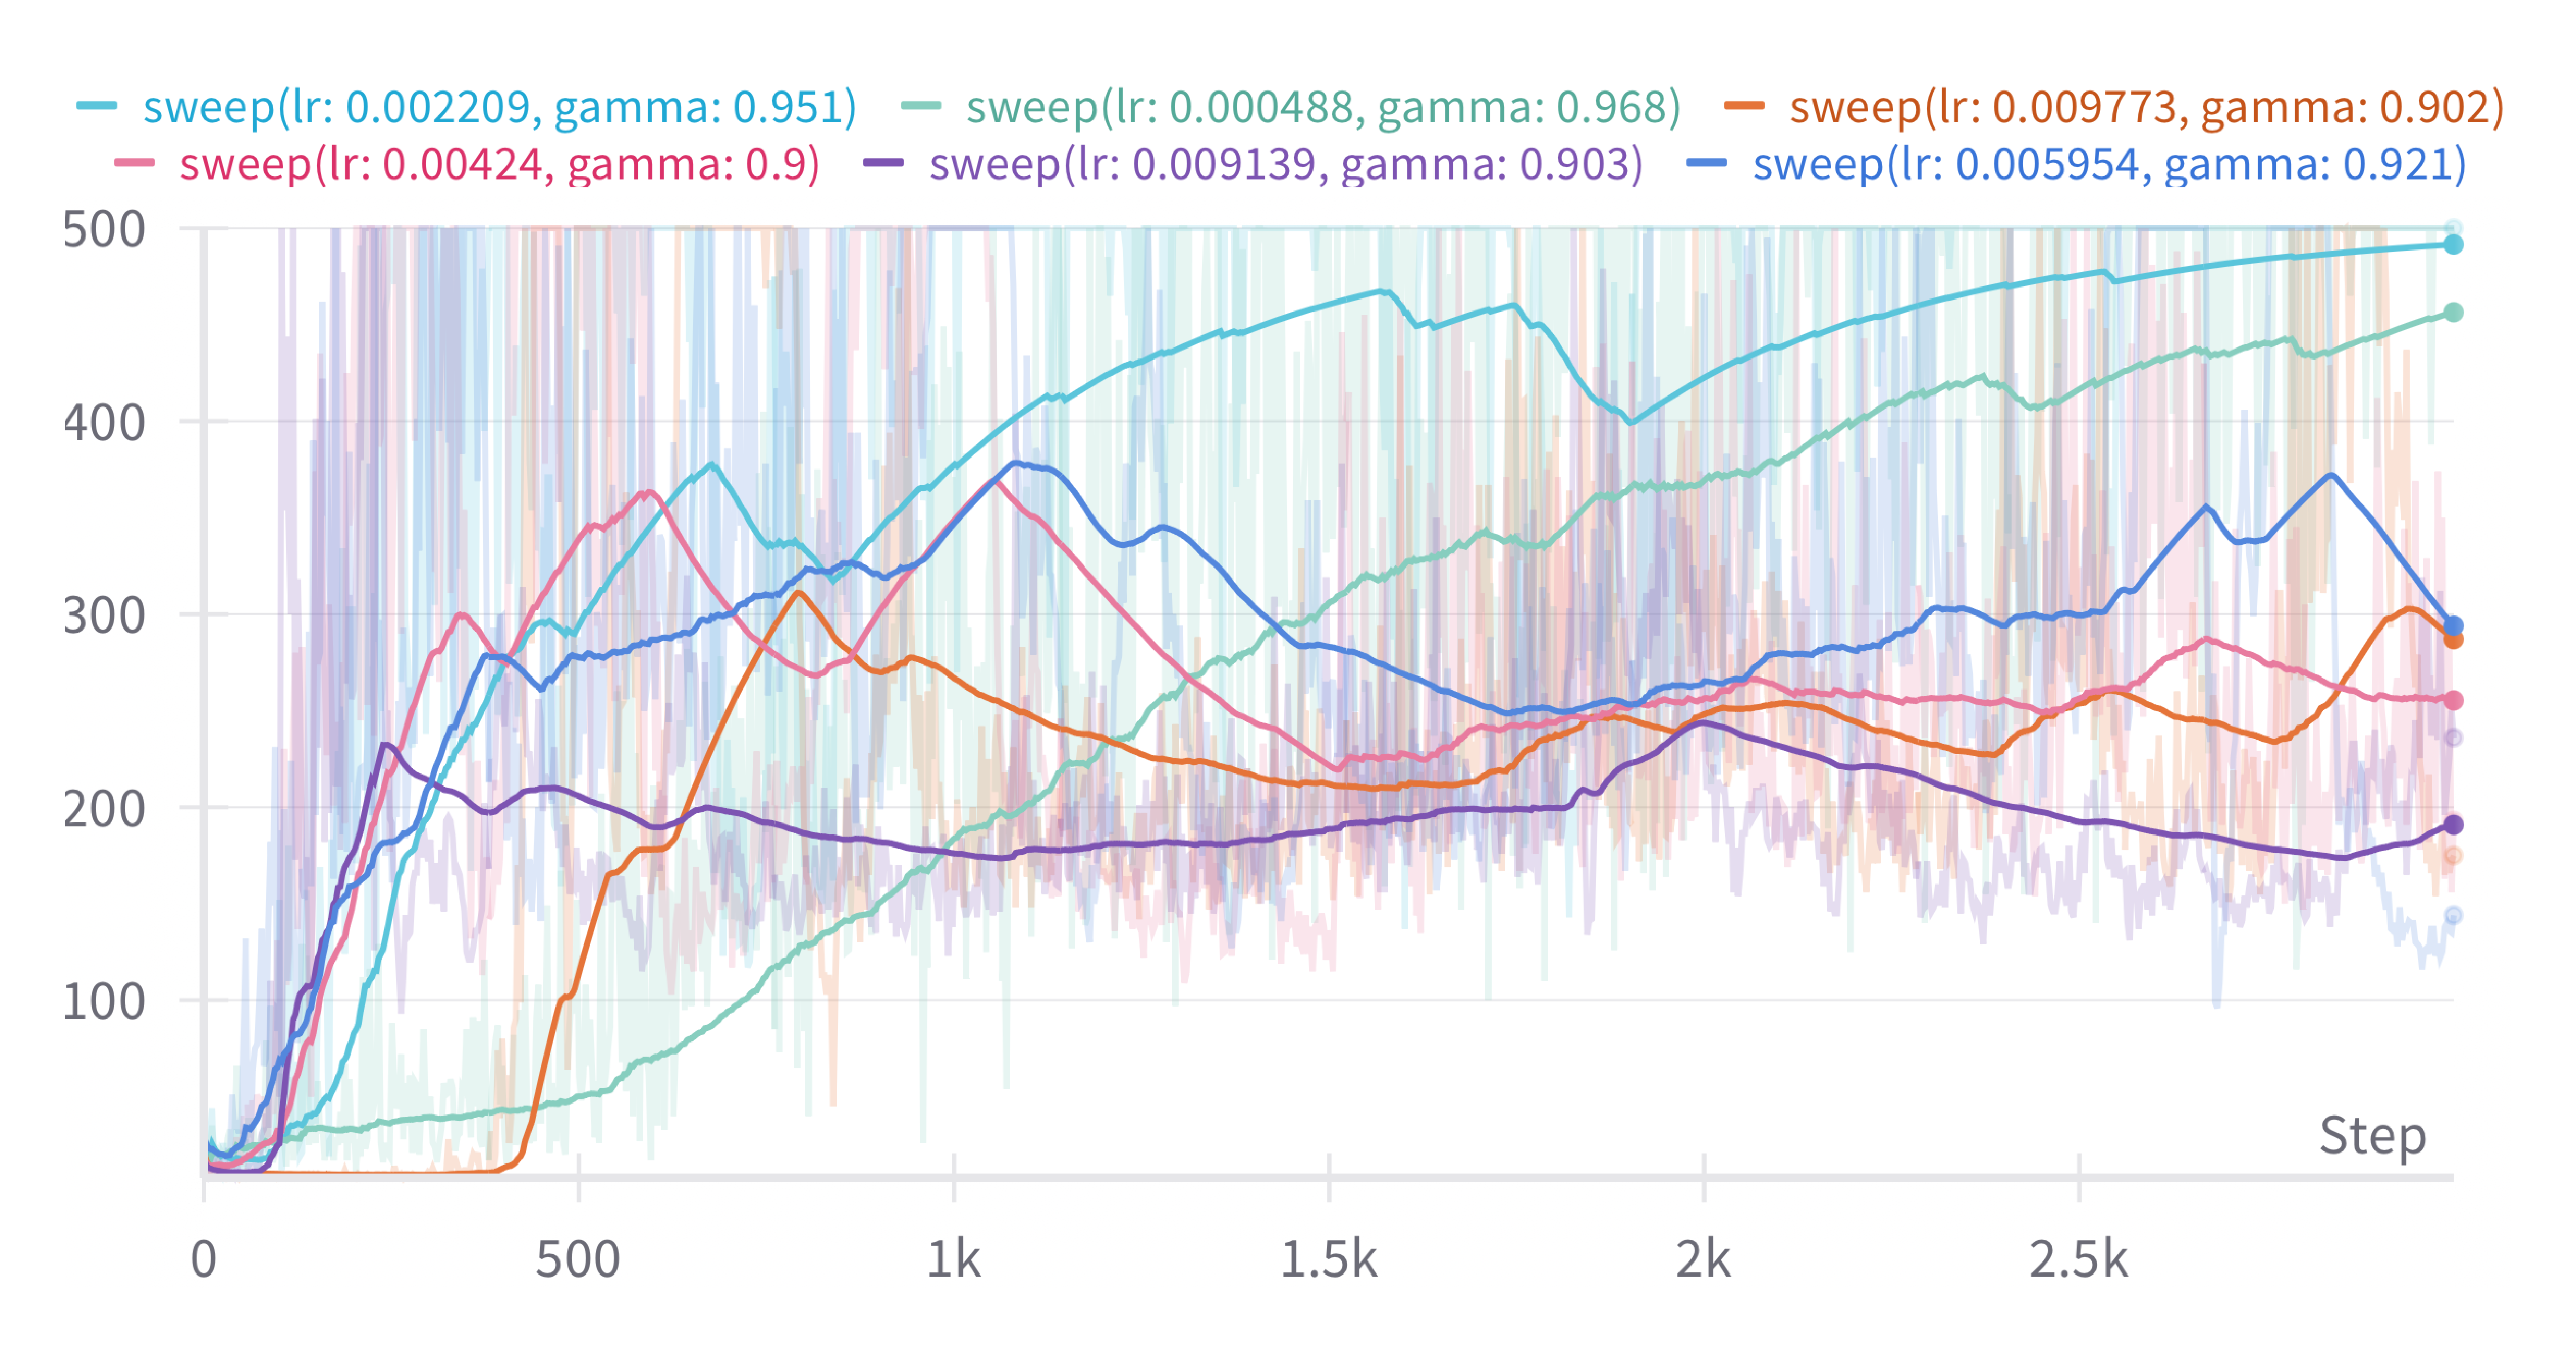
\includegraphics[width=.9\textwidth]{immages/3-cart pole/migliori.pdf}
\caption{Sweep su $\gamma$ e learning rate.}
\label{fig:ampiorange}
\end{figure}

\myskip

In Figura \ref{fig:migliorimale}, osserviamo che valori bassi di $\gamma$ impediscono la risoluzione dell’ambiente. Al contrario, come mostrato in Figura \ref{fig:miglioribene}, un $\gamma$ elevato migliora l’apprendimento. Learning rate più alti portano a una rapida risoluzione, ma con peggioramento successivo; learning rate più bassi rendono l’apprendimento più lento ma stabile.

\begin{figure}[htbp]
\centering
\begin{subfigure}{0.45\textwidth}
\centering
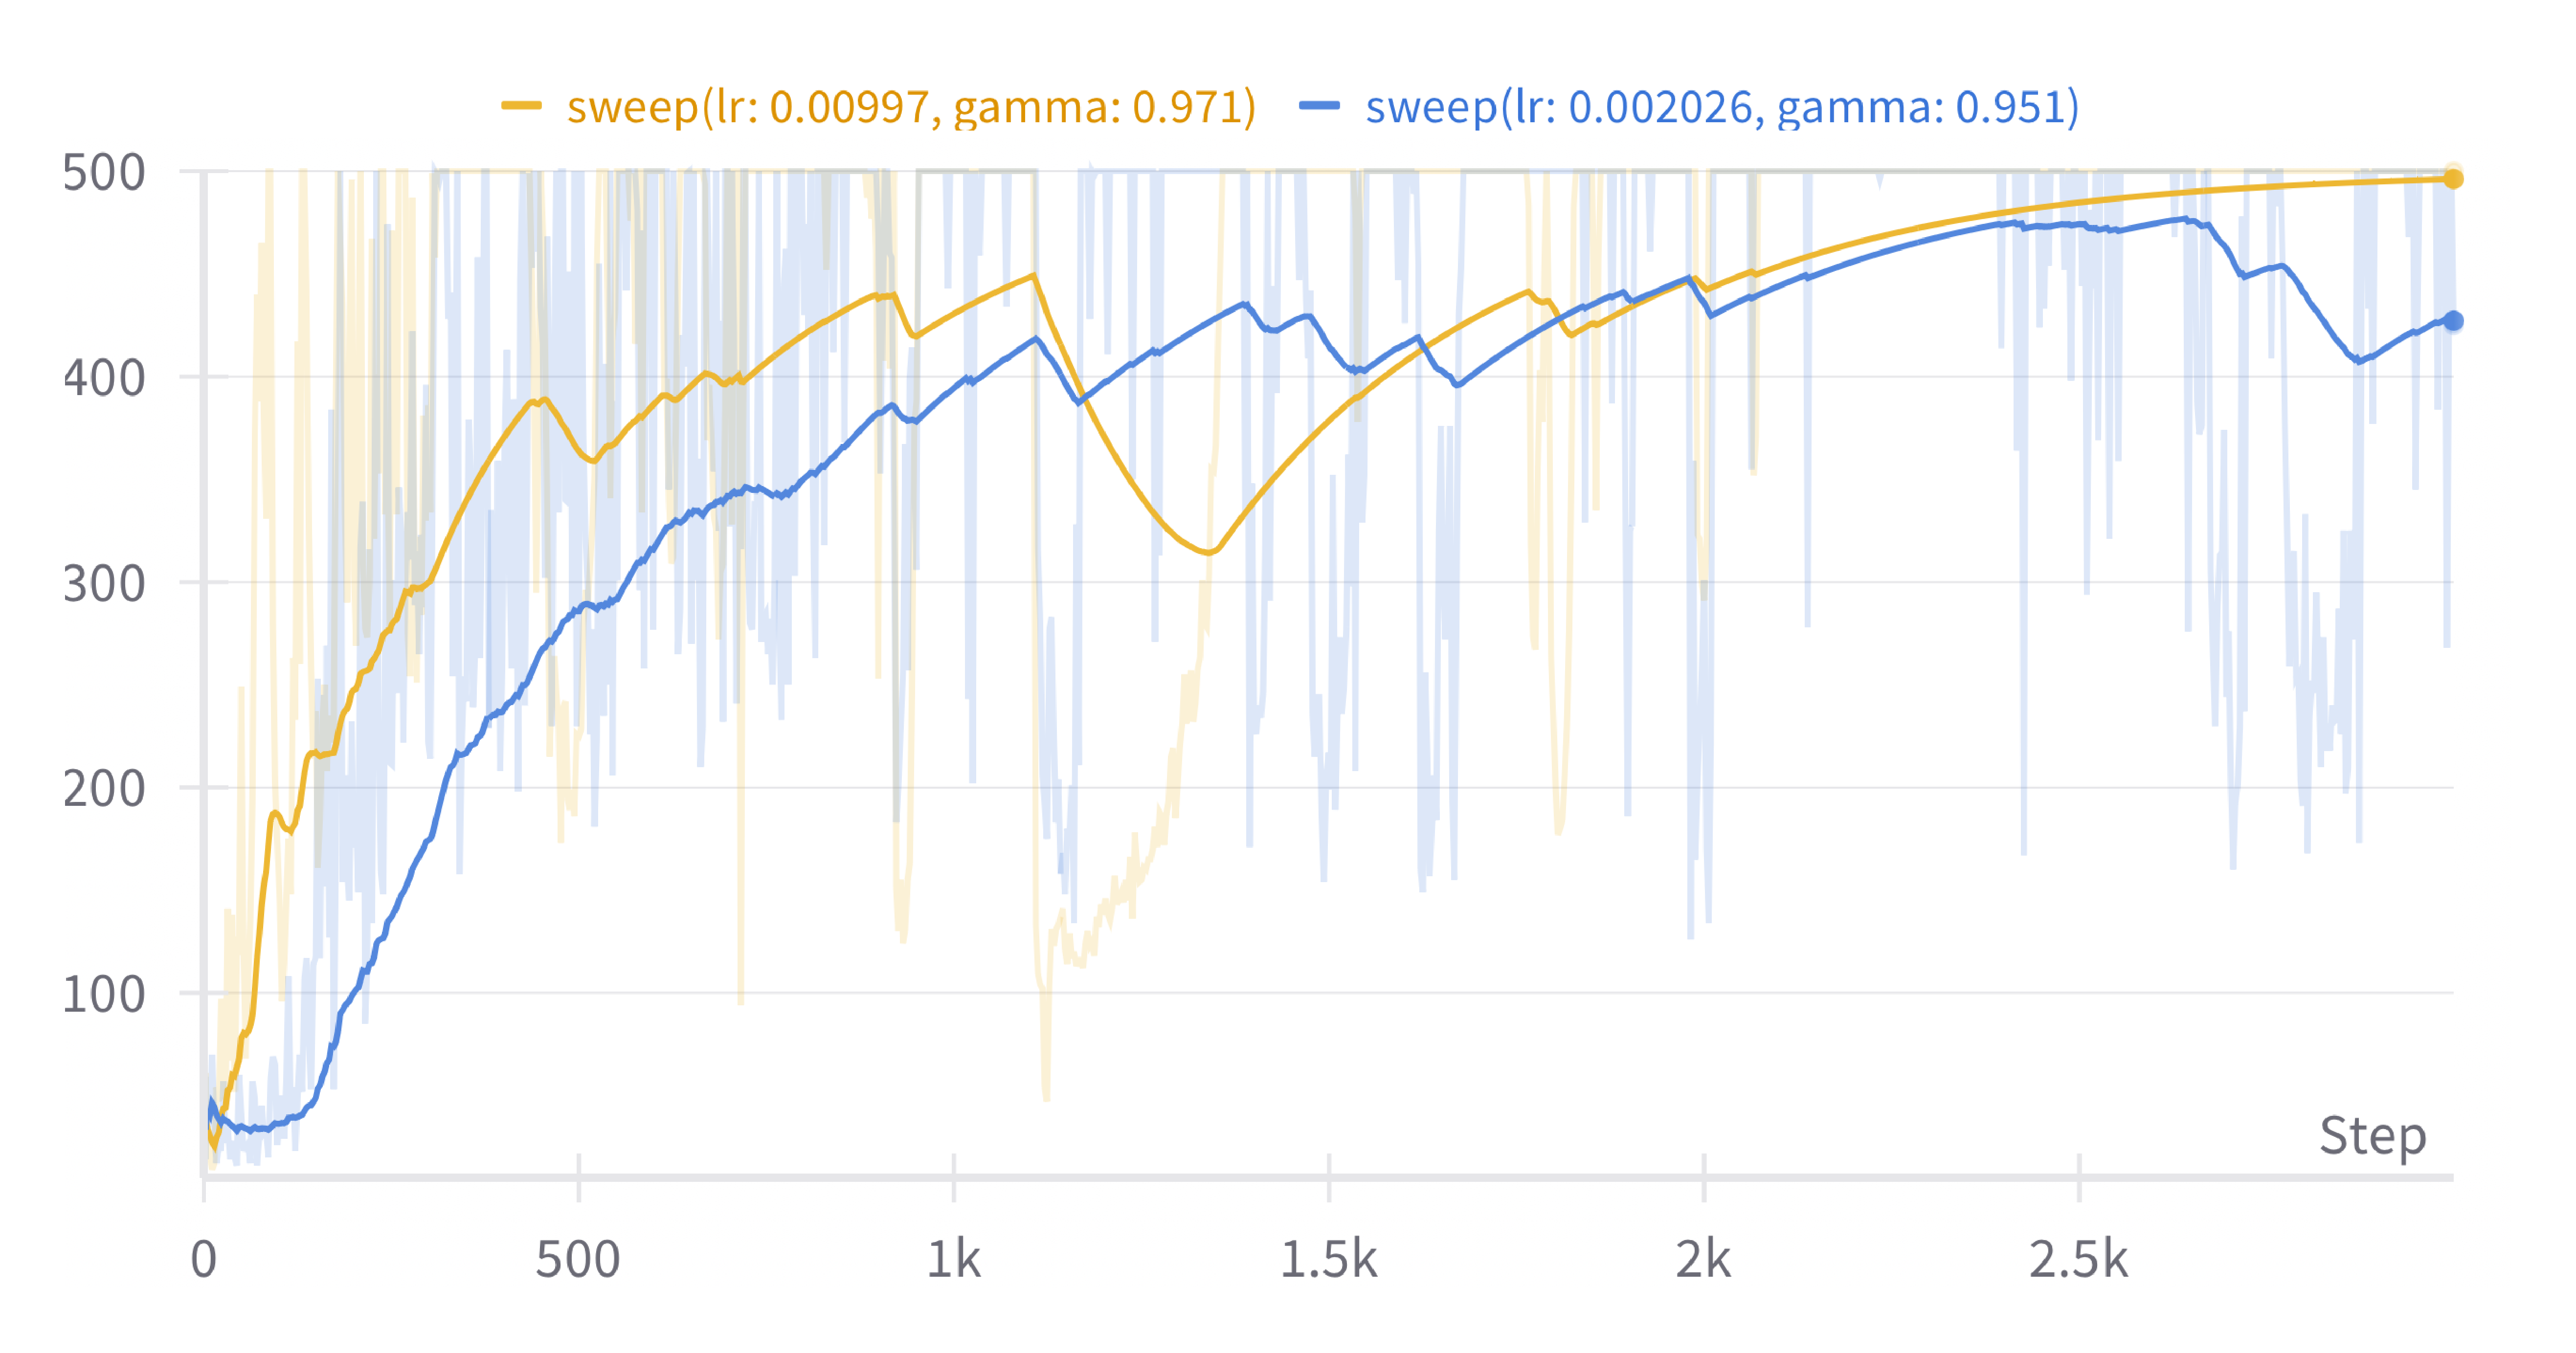
\includegraphics[width=.9\textwidth]{immages/3-cart pole/migliori_male.pdf}
\caption{$\gamma$ bassi}
\label{fig:migliorimale}
\end{subfigure}
\hfill
\begin{subfigure}{0.45\textwidth}
\centering
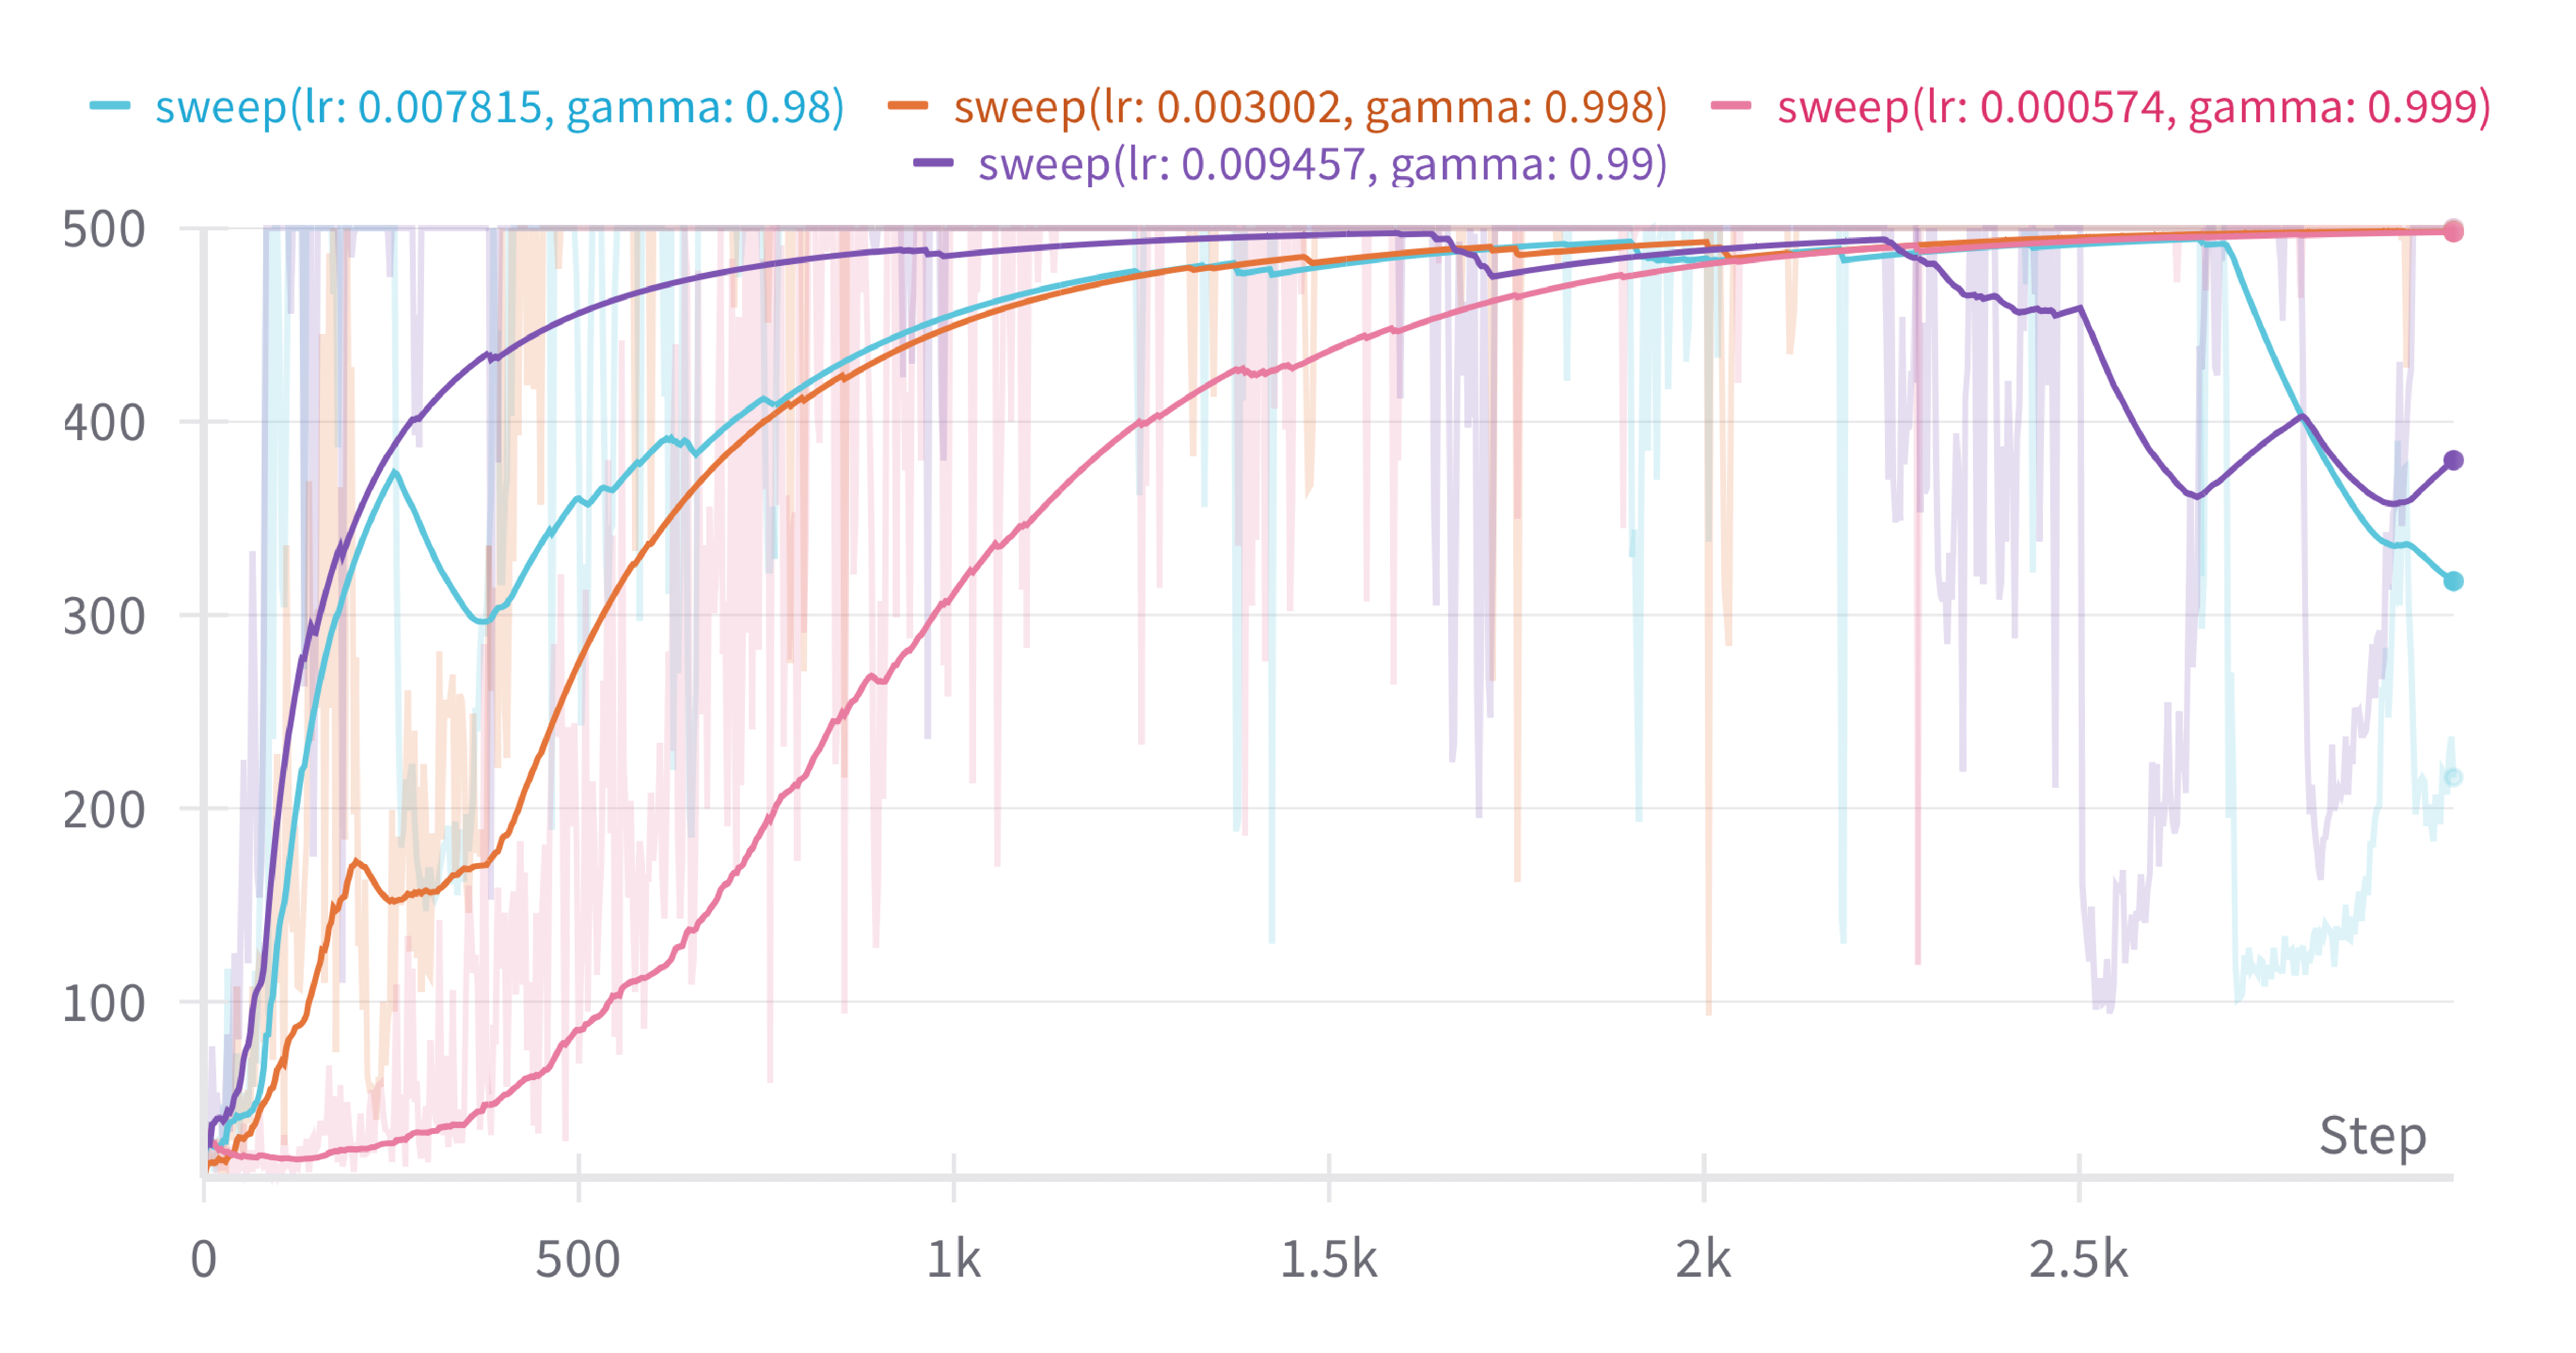
\includegraphics[width=\textwidth]{immages/3-cart pole/migliori_bene.pdf}
\caption{$\gamma$ alti}
\label{fig:miglioribene}
\end{subfigure}
\caption{Confronti tra esperimenti.}
\end{figure}